\documentclass[11pt,letterpaper]{article}
\usepackage[lmargin=1in,rmargin=1in,tmargin=1in,bmargin=1in]{geometry}
\usepackage{../style/homework}
\usepackage{../style/commands}
\setbool{quotetype}{true} % True: Side; False: Under
\setbool{hideans}{true} % Student: True; Instructor: False

% -------------------
% Content
% -------------------
\begin{document}

\homework{7: Due 03/03}{Today is a good day to try.}{Quasimodo, The Hunchback \par of Notre Dame}

% Problem 1
\problem{10} Being as accurate as possible, sketch the graph of the line $2x - 3y= 12$.
	\[
	\fbox{
	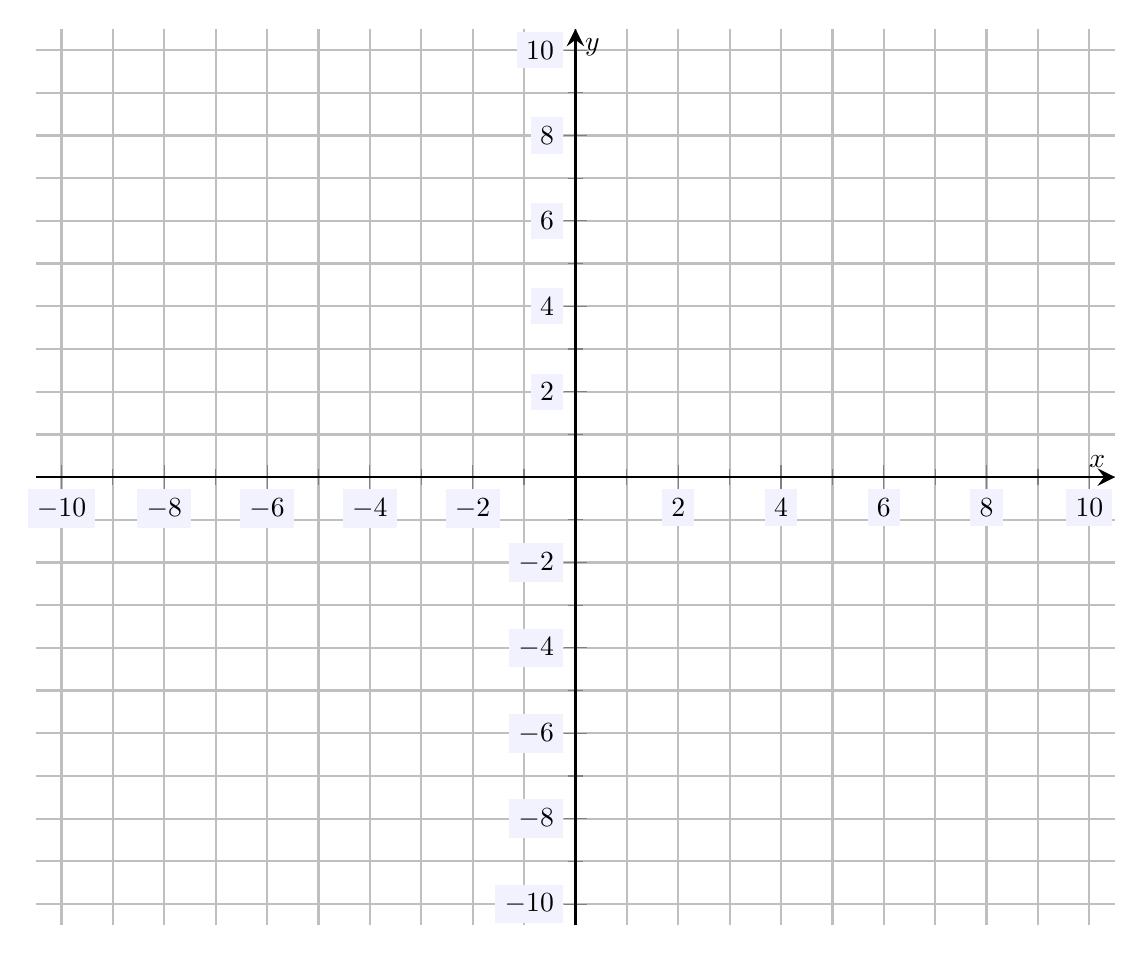
\begin{tikzpicture}[scale=2,every node/.style={scale=0.5}]
	\begin{axis}[
	grid=both,
	axis lines=middle,
	ticklabel style={fill=blue!5!white},
	xmin= -10.5, xmax=10.5,
	ymin= -10.5, ymax=10.5,
	xtick={-10,-8,-6,-4,-2,0,2,4,6,8,10},
	ytick={-10,-8,-6,-4,-2,0,2,4,6,8,10},
	minor tick = {-10,-9,...,10},
	xlabel=\(x\),ylabel=\(y\),
	]
	\end{axis}
	\end{tikzpicture}
	}
	\]



\newpage



% Problem 2
\problem{10} Consider the linear function $f(x)= 5 - \frac{3}{4}\,x$.
	\begin{enumerate}[(a)]
	\item Find the slope of this linear function. 
	\item Interpret the slope two different ways.
	\item Is the linear function increasing, decreasing, or constant? Explain. 
	\item Determine the $y$-intercept for $f(x)$.
	\item Determine the $x$-intercept for $f(x)$.
	\end{enumerate}



\newpage



% Problem 3
\problem{10} Showing all your work, find the equation of the line perpendicular to $y= 5 - 3x$ that passes through the point $(1, -4)$. 



\newpage



% Problem 4
\problem{10} Showing all your work, solve the following linear equation, be sure to verify that your solution satisfies the equation: 
	\[
	5x - 6= 1 - 7x
	\]



\newpage



% Problem 5
\problem{10} Water is flowing into a `rectangular' box with side lengths 2~ft, 4~ft, and 5~ft at a rate of 3.4~ft$^3$/min. Currently, the box contains 16~ft$^3$ of water. Let $W(t)$ denote the amount of water in the box $t$ minutes from now.
	\begin{enumerate}[(a)]
	\item Explain why $W(t)$ is linear.
	\item Find $W(t)$. 
	\item What do the slope and $y$-intercept of $W(t)$ represent in context?
	\item Determine when the box will begin to overflow. 
	\end{enumerate}


\end{document}